\documentclass[11pt]{article}

\usepackage{enumitem}
\usepackage{amsmath}
\usepackage{amssymb}
\usepackage{bm}
\usepackage{listings}
\usepackage{color}
\usepackage{tikz}
\usepackage[T1]{fontenc}
\usepackage{courier}
\usepackage{circuitikz}
\usetikzlibrary{calc}
\usepackage{changepage}
\usepackage{multirow}
\usepackage[margin=1.0in]{geometry}

\lstset{xleftmargin=-1cm,
	xrightmargin=\parindent,
	numbersep=5pt} 

\definecolor{dkgreen}{rgb}{0,0.6,0}
\definecolor{gray}{rgb}{0.5,0.5,0.5}
\definecolor{mauve}{rgb}{0.58,0,0.82}

\lstset{
	frame=tb,
	language=Verilog,
	aboveskip=3mm,
	belowskip=3mm,
	showstringspaces=false,
	columns=flexible,
	basicstyle={\small\ttfamily},
	numbers=none,
	numberstyle=\tiny\color{gray},
	keywordstyle=\color{blue},
	commentstyle=\color{dkgreen},
	stringstyle=\color{mauve},
	breaklines=true,
	breakatwhitespace=true,
	tabsize=3,
	xleftmargin=0pt,
}

\tikzset{
	multiplexer4/.pic = {
		
		% frame
		\draw[pic actions] (0, 0) coordinate (-NW) -- ++(300 : 1.5)
		coordinate (-SW) -- ++(0 : 1.5) coordinate (-SE) -- ++(60 : 1.5)
		coordinate (-NE) -- cycle;
		
		% output
		\coordinate (-output) at ($(-SW)!0.5!(-SE)$);
		
		% select
		\foreach \x/\lbl in {0.33/A,0.66/B} {
			\coordinate (-\lbl) at ($(-SE)!\x!(-NE)$);
			
		}
		
		% input
		\pgfmathsetmacro{\ymin}{0.75}
		\pgfmathsetmacro{\ymax}{2.25}
		\foreach \i in {0,1} {
			\foreach \j in {0,1} {
				\pgfmathsetmacro{\y}{\ymax - (\ymax - \ymin)*(2*\i + \j) / 3.};
				\coordinate (-\i\j) at (\y,0);
				\node[yshift = -8pt] at (-\i\j) {$\i\j$};
			}
		}
	}
}
\tikzset{
	multiplexer2/.pic = {
		\draw[pic actions] (0,0) coordinate (-NW) -- ++(300 : 0.8)
		coordinate (-SW) -- ++(0 : 0.8) coordinate (-SE) -- ++(60 : 0.8)
		coordinate (-NE) -- cycle;
		
		\coordinate (-output) at ($(-SW)!0.5!(-SE)$);
		
		\coordinate (-sel) at ($(-SE)!0.5!(-NE)$);
		
		\draw ($(-NW)!0.33!(-NE)$) -- ++(90 : 0.3) coordinate(-in0);
		\draw ($(-NW)!0.67!(-NE)$) -- ++(90 : 0.3) coordinate(-in1);
		\draw ($(-SW)!0.5!(-SE)$) -- ++(270 : 0.3) coordinate(-out);
		
		\node[yshift = -8pt] at ($(-NW)!0.33!(-NE)$) {$0$};
		\node[yshift = -8pt] at ($(-NW)!0.67!(-NE)$) {$1$};
	}	
}

\tikzset{
	alumux/.pic = {
		\draw (0,0) pic(-mpx1) [draw, fill=white] {multiplexer2};
		\draw (1.6,0) pic(-mpx2) [draw, fill=white] {multiplexer2};
		\draw (3.2,0) pic(-mpx3) [draw, fill=white] {multiplexer2};
		%\draw (4.8,0) pic(mpx4) [draw, fill=white] {multiplexer2};
		\draw (6.4,0) pic(-mpx5) [draw, fill=white] {multiplexer2};
		%\draw (8.0,0) pic(mpx6) [draw, fill=white] {multiplexer2};
		%\draw (9.6,0) pic(mpx7) [draw, fill=white] {multiplexer2};
		%\draw (11.2,0) pic(mpx8) [draw, fill=white] {multiplexer2};
		
		\draw (0.8,-2) pic(-mpx9) [draw, fill=white] {multiplexer2};
		\draw (4.0,-2) pic(-mpx10) [draw, fill=white] {multiplexer2};
		\draw (7.2,-2) pic(-mpx11) [draw, fill=white] {multiplexer2};
		\draw (10.4,-2) pic(-mpx12) [draw, fill=white] {multiplexer2};
		
		\draw (2.4,-4) pic(-mpx13) [draw, fill=white] {multiplexer2};
		\draw (8.8,-4) pic(-mpx14) [draw, fill=white] {multiplexer2};
		
		\draw (5.6,-6) pic(-mpx15) [draw, fill=white] {multiplexer2};
		
		\draw (-mpx1-out) -- (-mpx9-in0);
		\draw (-mpx2-out) -- (-mpx9-in1);
		\draw (-mpx3-out) -- (-mpx10-in0);
		%\draw (mpx4-out) -- (mpx10-in1);
		\draw (-mpx5-out) -- (-mpx11-in0);
		%\draw (mpx6-out) -- (mpx11-in1);
		%\draw (mpx7-out) -- (mpx12-in0);
		%\draw (mpx8-out) -- (mpx12-in1);
		
		\draw (-mpx9-out) -- (-mpx13-in0);
		\draw (-mpx10-out) -- (-mpx13-in1);
		\draw (-mpx11-out) -- (-mpx14-in0);
		\draw (-mpx12-out) -- (-mpx14-in1);
		
		\draw (-mpx13-out) -- (-mpx15-in0);
		\draw (-mpx14-out) -- (-mpx15-in1);
		
		\draw ($(-mpx1-SW)!0.5!(-mpx1-NW)$) -- ++(180 : 0.5) node[left]{$\texttt{op[0]}$};
		\draw ($(-mpx9-SW)!0.5!(-mpx9-NW)$) -- ++(180 : 0.5) node[left]{$\texttt{op[1]}$};
		\draw ($(-mpx13-SW)!0.5!(-mpx13-NW)$) -- ++(180 : 0.5) node[left]{$\texttt{op[2]}$};
		\draw ($(-mpx15-SW)!0.5!(-mpx15-NW)$) -- ++(180 : 0.5) node[left]{$\texttt{op[3]}$};
		
		\node[above, right, rotate=90] at (-mpx1-in0) {$\texttt{sub\_val}$};
		\node[above, right, rotate=90] at (-mpx1-in1) {$\texttt{add\_val}$};
		\node[above, right, rotate=90] at (-mpx2-in0) {$\texttt{or\_val}$};
		\node[above, right, rotate=90] at (-mpx2-in1) {$\texttt{and\_val}$};
		\node[above, right, rotate=90] at (-mpx3-in0) {$\texttt{dec\_val}$};
		\node[above, right, rotate=90] at (-mpx3-in1) {$\texttt{inc\_val}$};
		\node[above, right, rotate=90] at (-mpx10-in1) {$\texttt{inv\_val}$};
		\node[above, right, rotate=90] at (-mpx5-in0) {$\texttt{lsl\_val}$};
		\node[above, right, rotate=90] at (-mpx5-in1) {$\texttt{slt\_val}$};
		\node[above, right, rotate=90] at (-mpx11-in1) {$\texttt{lsr\_val}$};
		\node[above, right, rotate=90] at (-mpx12-in0) {$\texttt{asl\_val}$};
		\node[above, right, rotate=90] at (-mpx12-in1) {$\texttt{asr\_val}$};
		
		\node[below] at (-mpx15-out) {$\texttt{ovf,out}$};
	}
}

\title{CS152B Lab 1}

\begin{document}
	
\title{\vspace{-1.0in} Com Sci 152B Digital Design \\
	Lab 1: ALU \& Register File Implementation }
\date{}
\maketitle
\vspace{-0.75in}
\begin{center}
\begin{tabular}{cc}
	Michael Hale & 004-620-459 \\ 
	Matthew Nuesca & 904-440-067 \\ 
	Shilin Patel & 904-569-866 \\ 
	Bingxin Zhu & 704-845-969
\end{tabular}
\end{center}

\section{Overview}

In this lab we implemented two key components found in modern processors: the arithmetic logic unit (ALU) and the register file. The purpose of the ALU is to perform a variety of operations on arbitrary 16-bit integers and write the result to an output port. On the other hand, the register file performs no computation and simply reads and writes to a series of internal 16-bit registers. 

\section{Design Requirements}
\subsection{ALU Requirements}
The ALU shall perform a set of logical and arithmetic operations given the sixteen bit inputs \texttt{a} and \texttt{b} and the four bit op-code \texttt{op}. The ALU must write the output of the encoded operation to a sixteen bit output \texttt{out} and set two flags (\texttt{ovf,zero}) if the operation results in overflow or a zero output respectively. 

The operations to be encoded are: \\

{\centering
\begin{tabular}{|c|l|c|}
	\hline
	\textbf{OP} & \textbf{Description} & \textbf{Symbolically}\\
	\hline
	0000 & Subtraction & $a - b$ \\
	0001 & Addition & $a + b$ \\
	0010 & Bitwise OR & $a~|~b$ \\
	0011 & Bitwise AND & $a~\&~b$ \\
	0100 & Decrement & $a - 1$ \\
	0101 & Increment & $a + 1$ \\
	0110 & Inverse & $\sim a$ \\
	1000 & Logical left shift & $a << b$ \\
	1001 & Set on less than or equal & $a \leq b$ \\
	1010 & Logical right shift & $a >> b$ \\
	1100 & Arithmetic left shift & $a <<< b$ \\
	1110 & Arithmetic right shift & $a >>> b$ \\
	\hline
\end{tabular} \par
} 

\vspace{12pt}
Table 1: Specifications for each operation.

\subsection{Register File Requirements}
The register file shall contain 32 sixteen bit registers and must include two sixteen bit read ports and a write port (\texttt{bus\_a, bus\_b, write\_bus}) with their corresponding five bit register select ports (\texttt{ra, rb, rw}). It must also accept a write-enable signal (\texttt{wren}), a clock signal (\texttt{clk}) and a reset signal (\texttt{rst}) which sets the contents of each register to zero. Additionally, if a register is being read and written at the same time, the read should reflect the updated value immediately. 

\section{Implementation}
\subsection{ALU Implementation}
Our ALU implementation essentially partitions each instruction into a single Verilog module. In the top level ALU module, the inputs \texttt{a} and \texttt{b} fan out into each of these instruction modules which each independently generate an \texttt{ovf} and \texttt{result} signal concatenated into a single \texttt{out} signal. These signals are then fed into a multiplexer which uses the op-code \texttt{op} to determine the ALU output. The \texttt{zero} flag is generated by OR-ing each bit of the output and inverting the result.

\subsubsection{Output Multiplexer}
Rather than designing a single multiplexer that would take 12 seventeen bit inputs and generate one seventeen bit output, we instead created a simple two-input multiplexer module. In our top level ALU module, we then instantiated arrays of these muxes of length 17 to handle the wide instruction outputs. To generalize the multiplexer to 12 inputs, we created a cascade of 2-input muxes where each stage was determined by a different bit of the op-code \texttt{op}. Figure 1 shows how each bit of the op-code selects a level of the hierarchy of muxes. \\

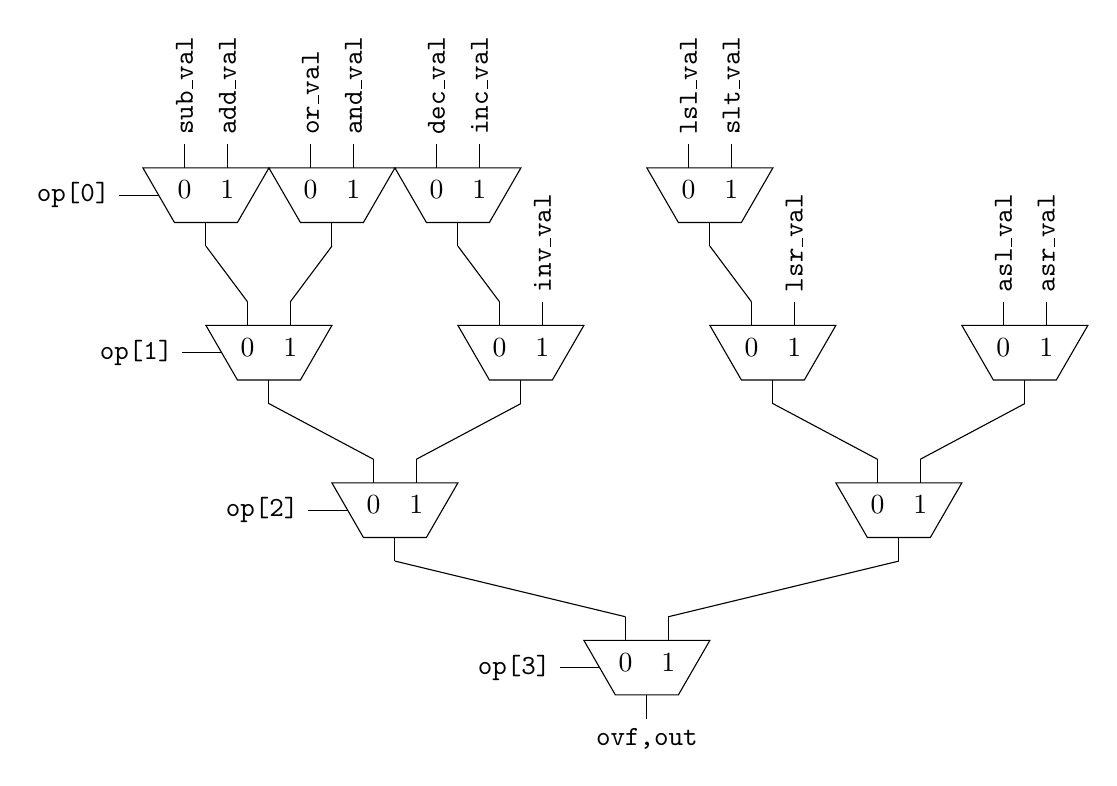
\begin{tikzpicture}
\draw pic() [draw, scale=1.0] {alumux};
\end{tikzpicture}

Figure 1: Tree of 2-input muxes to mimic the operation of a 16-input mux.

\subsubsection{Addition Implementation} 
The ADD, SUB, INC, DEC, and SLT instructions are implemented using the adder module. The adder performs 16-bit two's-complement addition and concatenates the \texttt{ovf} bit to the front of the 16-bit \texttt{sum}. Our design is a simple implementation of a ripple-carry adder, with the 1-bit adder implemented in a separate module. 

The 1-bit adder logic uses propagate (\texttt{p}) and generate (\texttt{g}) intermediate signals to determine the outputs \texttt{co} and \texttt{sum}.

\begin{lstlisting}
input a, b, ci;
output sum, co;

wire p = a | b;
wire g = a & b;

assign co = g | (ci & p);
assign sum = ci ^ a ^ b;
\end{lstlisting}

This allows us to connect the carry signals with a single line of Verilog code in the 16-bit adder module.

\begin{lstlisting}
input [15:0] a, b;
input ci;
output [16:0] out;

wire[15:0] sum;
wire[16:0] carry;
assign carry[0] = ci;

addbit adders[15:0](a,b,carry[15:0],sum,carry[16:1]);
\end{lstlisting}

Finally our overflow logic checks the two cases where the input signs are the same, and the sign of the sum differs. This bit is then concatenated to the front of the output.

\begin{lstlisting}
assign overflow = (~sum[15] & a[15] & b[15]) 
	|| (sum[15] & ~a[15] & ~b[15]);
assign out = {overflow,sum};
\end{lstlisting}

\subsubsection{Other Instruction Modules}
Each of the other instructions (logical shifts, arithmetic shifts, and bitwise operations) can be implemented using the permitted Verilog built-in operations (\texttt{$<<$,$>>$,$<<<$,$>>>$,\&,|,\sim}).

\subsection{Register File Implementation}
The register file contains 32 16-bit registers, each initialized to zero. Upon receiving a positive clock edge, the reset bit is first checked and honored. If the reset signal is low, we perform two actions:
\begin{enumerate}
	\item If the \texttt{wren} bit is high, we read from the \texttt{write\_bus} and write to the register designated by \texttt{rw}.
	
	\item We read from the registers designated by \texttt{ra} and \texttt{rb} unless a simultaneous write is taking place.
\end{enumerate}

This behavior is implemented with the following Verilog code:
\begin{lstlisting}
// Honor the reset signal
if (rst == 1) begin
	for (idx=0; idx < 32; idx=idx+1) begin
		registers[idx] <= 16'b0;
	end
end else begin
// Write to register rw
if (wren == 1) begin
	registers[rw] <= write_bus;
end 
// Read from register ra
if (wren == 1 && ra == rw) begin
	bus_a <= write_bus;
end else begin
	bus_a <= registers[ra];
end
// Read from register rb
if (wren == 1 && rb == rw) begin
	bus_b <= write_bus;
end else begin
	bus_b <= registers[rb];
end
\end{lstlisting}

\section{Testbench}
\subsection{ALU Testing}
We tested the ALU by hard coding a series of test cases for each instruction and checking the output. If the output does not match the expected output, the failure will be printed to the console. Some instructions required us to dedicate more test cases, by the nature of their edge cases. Below is a comprehensive table of the test cases for each instruction: \\

{\centering
\begin{tabular}{|c|l|l|l|l|}
	\hline
	\textbf{Operation} & \textbf{Input $A$} & \textbf{Input $B$} & \textbf{Output} & \textbf{Overflow} \\
	\hline
	
	\multirow{7}{*}{Subtraction} & 91 & 47 & 44 & 0 \\
	& -91 & -47 & -44 & 0 \\
	& 91 & 100 & -9 & 0 \\
	& -50 & -132 & 82 & 0 \\
	& 30000 & -3456 & X & 1 \\
	& -32000 & 10000 & X & 1 \\
	& -15 & -15 & 0 & 0 \\
	\hline
	
	\multirow{6}{*}{Addition} & 15 & 19 & 34 & 0 \\
	& -20 & -144 & -164 & 0 \\
	& 15 & -19 & -4 & 0 \\
	& -15 & 19 & 4 & 0 \\
	& 31748 & 1020 & X & 1 \\
	& -30851 & -1918 & X & 1 \\
	\hline
	
	\multirow{3}{*}{Bitwise OR} & 0x55AA & 0xAA55 & 0xFFFF & 0 \\
	& 0x00FF & 0xAA55 & 0xAAFF & 0 \\
	& 0x00FF & 0x0FF0 & 0x0FFF & 0 \\
	\hline
	
	\multirow{3}{*}{Bitwise AND} & 0x55AA & 0xAA55 & 0x0000 & 0 \\
	& 0x55AA & 0x00FF & 0x00AA & 0 \\
	& 0x55AA & 0x55AA & 0x55AA & 0 \\
	\hline
\end{tabular} \par
}

{\centering
\begin{tabular}{|c|l|l|l|l|}
	\hline
	\textbf{Operation} & \textbf{Input $A$} & \textbf{Input $B$} & \textbf{Output} & \textbf{Overflow} \\
	\hline
	
	\multirow{3}{*}{Decrement} & 21930 & X & 21929 & 0 \\
	& 0 & X & -1 & 0 \\
	& -32768 & X & X & 1 \\
	\hline
	
	\multirow{3}{*}{Increment} & 21930 & X & 21931 & 0 \\
	& -1 & X & 0 & 0 \\
	& 32767 & X & X & 1 \\
	\hline
	
	\multirow{3}{*}{Bitwise INV} & 0x0000 & X & 0xFFFF & 0 \\
	& 0x55AA & X & 0xAA55 & 0 \\
	& 0xFFFF & X & 0x0000 & 0 \\
	\hline
	
	\multirow{3}{*}{Logical Shift Left} & 0x55AA & 1 & 0xAB54 & 0 \\
	& 0x55AA & 16 & 0x0000 & 0 \\
	& 0x55AA & 0 & 0x55AA & 0 \\
	\hline
	
	& 36 & 45 & 1 & 0 \\
	& 36 & 15 & 0 & 0 \\
	Set on Less Than & 32767 & -2 & 0 & 0 \\
	Or Equal & -10 & 10 & 1 & 0 \\
	& 10 & -10 & 0 & 0 \\
	& -32768 & 1 & 1 & 0 \\
	& 10 & 10 & 1 & 0 \\
	\hline
	
	\multirow{3}{*}{Logical Right Shift} & 0x55AA & 1 & 0x2AD5 & 0 \\
	& 0x55AA & 16 & 0x0000 & 0 \\
	& 0x55AA & 0 & 0x55AA & 0 \\
	\hline
	
	\multirow{3}{*}{Arithmetic Left Shift} & 0x55AA & 1 & 0xAB54 & 1 \\
	& 0xF000 & 16 & 0x0000 & 1 \\
	& 0xAA55 & 0 & 0xAA55 & 0 \\
	\hline
	
	\multirow{3}{*}{Arithmetic Right Shift} & 0xAA55 & 1 & 0xD52A & 0 \\
	& 0xAA55 & 16 & 0xFFFF & 0 \\
	& 0xAA55 & 0 & 0xAA55 & 0 \\
	\hline
\end{tabular} \par 
}

\vspace{12pt}
Table 2: Test cases.

\subsection{Register File Testing}
To test the register file, we first write to each register the value 0x55AA individually. We then loop through and read from each register (two at a time) to verify that the contents match the written value. In the other test, we write to $R_0$ at the same time that we are reading from $R_0$ and $R_1$, verifying that the read is updated instantly. 

\section{Challenges \& Solutions}

\section{Questions}
\begin{enumerate}
	\item \textbf{What is the difference between structural and behavioral Verilog? Please provide an example of a structural and behavioral implementation of a multiplexer.} 
	
	Structural Verilog is an implementation of a system using only basic module building blocks, such as logic gates. No logic abstracted further than wires and gates is allowed. Behavioral Verilog can implement abstractions on top of logic gates such as conditionals and looping. Behavioral Verilog also may rely on always blocks to abstract clock edge based operations that in structural Verilog would require far more effort to manipulate. Using this type of syntax may limit knowledge of what is actually occurring on the hardware (as is natural with every abstraction).
	
	Implementation of a multiplexer using structural Verilog:
	
	\begin{lstlisting}
	input select_bit, input_a, input_b;
	output out;
	
	//Structural multiplexer (only uses logic gates):
	assign out = (input_a & !select_bit) | 
	                  (input_b & select_bit);
	\end{lstlisting}
	
	Implementation of a multiplexer using behavioral Verilog:
	
	\begin{lstlisting}
	input select_bit, input_a, input_b;
	output reg out;
	
	//Behavioral multiplexer (uses abstracted logic):	
	always @ (select_bit or input_a or input_b)	begin
		if (select_bit == 1'b0) begin
			out <= input_a;
		end else begin
			out <= input_b;
		end
	end
	\end{lstlisting}
	
	\item \textbf{What is the difference between an asynchronous and synchronous Multiplexer? Please provide a brief explanation on how you could implement both using behavioral Verilog.}
	
	An asynchronous multiplexer is the one implemented in the previous question. This approach is always checking for either input or select bits to determine which option to choose. The actual assignment of one of the inputs to the output is non blocking, meaning it will happen independent of the order of other operations occurring in the system. A synchronous mux implements the same logic but uses blocking assignments and doesn't necessitate an always block. It will run in a specific order with other modules and will complete at a known time. 
	
	Behavioral synchronous multiplexer:
	
	\begin{lstlisting}
	input select_bit, input_a, input_b;
	output out;
	
	assign out = select_bit ? input_a : input_b;
	\end{lstlisting}
	
	\item \textbf{What is the difference between an arithmetic and logical shifter?}
	
	The difference between the implementations of the shifters are determined by the characteristics of each shift. Arithmetic and logical left shifts are almost identical. When the bits are shifted left (towards the MSB), the now open position is filled with a 0. The difference is that the logical shift can not overflow, while the arithmetic shift will overflow if the new MSB is different from the previous MSB. Arithmetic right shifts shift towards the LSB, with the open position becoming a copy of the sign bit (if two's complement representation), or the MSB (in a general case). Logical right shift will be similar to the arithmetic right shift, except that the open bit will always be replaced by a zero, not the previous MSB. Shifts, arithmetic (<<<, >>>) and logical (<<, >>), are implemented using behavioral logic for this project, however the arithmetic overflow is determined by using an XOR on the MSB of the input and the MSB of the output. 
	
	\item \textbf{Assuming that you did NOT use Behavioral Verilog to implement an arithmetic shifter, how could you design one from scratch? Please include a simple diagram.}
	
	Using only structural components, let's implement an arithmetic right shifter. This is achievable using only multiplexers. Below is a diagram for a four bit shifter. The 2 to 1 multiplexer logic is abstracted to a black box using the implementation described above. There is no overflow for the right shift as the sign bit will never change.
	
	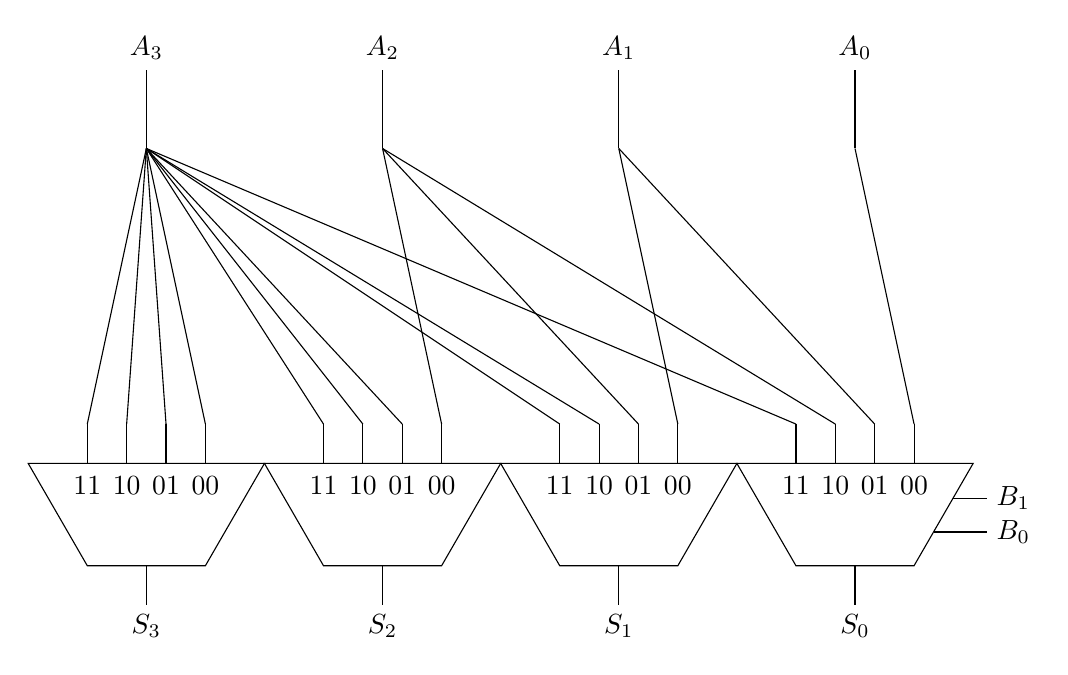
\begin{tikzpicture}
	
	\draw (0,0) pic(multi3) [draw, fill = white] {multiplexer4};
	\draw (3,0) pic(multi2) [draw, fill = white] {multiplexer4};
	\draw (6,0) pic(multi1) [draw, fill = white] {multiplexer4};
	\draw (9,0) pic(multi0) [draw, fill = white] {multiplexer4};
	
	% select
	\coordinate (T) at ([xshift = 5pt]multi0-NE);
	\draw (multi0-A) -- (multi0-A -| T) node[right]{$B_0$};
	\draw (multi0-B) -- (multi0-B -| T) node[right]{$B_1$};
	%\foreach \s in {A,B} 
	%\draw (multi1-\s) -- (multi1-\s -|  T) node[right]{$\s$};
	\coordinate (A0) at (10.5,5);
	\coordinate (A1) at (7.5,5);
	\coordinate (A2) at (4.5,5);
	\coordinate (A3) at (1.5,5);
	
	\coordinate (N0) at (10.5,4);
	\coordinate (N1) at (7.5,4);
	\coordinate (N2) at (4.5,4);
	\coordinate (N3) at (1.5,4);
	\foreach \a in {0,1,2,3}
	\draw (N\a) -- (A\a) node[above]{$A_\a$};
	\foreach \m in {0,1,2,3} {
		\foreach \i in {00,01,10,11} {
			\draw (multi\m-\i) -- ++(90:0.5) coordinate (multi\m-\i-raised);
		}	
	}
	\draw (multi0-00-raised) -- (N0);
	\draw (multi1-00-raised) -- (N1);
	\draw (multi0-01-raised) -- (N1);
	\draw (multi2-00-raised) -- (N2);
	\draw (multi1-01-raised) -- (N2);
	\draw (multi0-10-raised) -- (N2);
	\draw (multi3-00-raised) -- (N3);
	\draw (multi2-01-raised) -- (N3);
	\draw (multi1-10-raised) -- (N3);
	\draw (multi0-11-raised) -- (N3);
	
	\draw (multi3-11-raised) -- (N3);
	\draw (multi3-10-raised) -- (N3);
	\draw (multi3-01-raised) -- (N3);
	\draw (multi2-11-raised) -- (N3);
	\draw (multi2-10-raised) -- (N3);
	\draw (multi1-11-raised) -- (N3);
	
	% output
	\draw (multi3-output) -- ++(270:0.5) node[below]{$S_3$};
	\draw (multi2-output) -- ++(270:0.5) node[below]{$S_2$};
	\draw (multi1-output) -- ++(270:0.5) node[below]{$S_1$};
	\draw (multi0-output) -- ++(270:0.5) node[below]{$S_0$};
	
	\end{tikzpicture}
	
	Figure 2: Arithmetic right shifter.
	
\end{enumerate}

\end{document}